% !TEX root = ../../document.tex

\documentclass{subfiles}

\begin{document}

  \chapter{Métodos de Resolución}
  \label{chap:solving}

    \section{Introducción}
    \label{sec:solving_introduction}

      \paragraph{}
      Los problemas de \emph{optimización combinatoria} constituyen una de las categorías más interesantes dentro del área de la optimización de variables. Esto se debe a la gran aplicabilidad de los mismos en situaciones de la vida real, así como la gran reducción de costes que se puede alcanzar cuando estos son aplicados en los puntos estratégicos de cualquier proceso de producción.

      \paragraph{}
      Sin embargo, esta categoría de problemas de optimización presenta un mayor grado de dificultad en su resolución, tal y como se ha indicado a lo largo del \cref{chap:formulation}. Entre otros, esto se debe a la imposibilidad de utilizar técnicas basadas en gradientes (que en problemas con variables de decisión continuas proporcionan simplifican mucho su resolución). Puesto que estas técnicas no son aplicables, la estrategia alternativa se basa en la enumeración de posibles configuraciones de variables de manera inteligente hasta alcanzar aquella que genere el resultado óptimo para la instancia del problema que se pretenda resolver.

      \paragraph{}
      Por tanto, a pesar de no ser posible el apoyo en técnicas basadas en gradientes, si que existe la aternativa basada en enumeración de configuraciones como enfoque para dar con el óptimo. A pesar de ello, es fácil darse cuenta de que esta estrategia no es lo suficientemente potente como para permitir resolver problemas reales (o incluso de pequeño tamaño). La dificultad radica en la explosión combinatoria generada por la enumeración de soluciones. Por ejemplo, en un problema compuesto por $20$ variables de decisión de naturaleza binaria, el número de configuraciones a evaluar alcanzaría el valor de $2^{20} = 1048576$, lo cual no es escalable a problemas de gran tamaño, donde hay cientos o miles de variables de decisión con las que trabajar.

      \paragraph{}
      A pesar de esta dificultad, es posible enfrentarse a problemas de \emph{optimización combinatoria} de tamaños relativamente grande teniendo en cuenta distintas estrategias que permiten ignorar un gran número de configuraciones no factibles dadas las restricciones descritas por el problema en cuestión. Es por ello que muchos de los métodos de resolución se apoyan en estas garantias para enfocar la búsqueda sobre un subespacio de configuraciones factibles. Otra de las ideas más utilizadas por los métodos de resolución es apoyarse en los resultados de evaluación de configuraciones anteriores para que el coste computacional de evaluación de configuraciones actuales sea mucho menor. Dicha estrategia algorítmica se conoce como \emph{Programación Dinámica}, la cual se describe en mayor detalle en \cite{bellman1954theory}.


      \paragraph{}
      A lo largo del capítulo se decriben distintas situaciones en que es posible aplicar las técnicas anteriormente descritas sobre el \emph{problema Dial-a-Ride} para tratar de reducir en la medida de los posible la complejidad computacional que este presenta. Entonces, el resto del capítulo se organiza de la siguiente manera: En el \cref{sec:solving_exacts} se describen las distintas técnicas de resolución exactas que la literatura especializada en el problema a probado para tratar de resolver el problema. Seguidamente, en el \cref{sec:solving_heuristics} se describen estrategia basadas en heurísticas (tanto de construcción como mejora de soluciones) que a pesar de no ofrecer ninguna garantía de optimalidad, ofrecen un buen equilibrio entre tiempo de cómputo y calidad de las soluciones. Después, en el \cref{sec:solving_metaheuristics} se describen un conjunto de metaheurísticas basadas en la utilización de las heurísticas descritas en el apartado anterior de manera inteligente de tal manera que las configuraciones generadas proporcionan soluciones de mayor calidad. Por último, en el \cref{sec:solving_conclusions} se incluyen unas conclusiones generales acerca de los métodos de resolución aplicados al \emph{problema Dial-a-Ride}.

    \section{Métodos de Resolución Exactos}
    \label{sec:solving_exacts}

      \paragraph{}
      Los métodos de resolución exactos representan una de las categorías de resolución de problemas de optimización más interesantes debido a distintos factores, entre los que se encuentran aquellas situaciones en que es estrictamente necesario obtener el valor óptimo para una instancia dada. Sin embargo, esta categoría no solo es interesante por dicha razón, sino que el estudio de estos problemas además proporciona en muchas ocasiones razonamientos y justificaciones teóricas sobre el problema que pretenden resolver que ayudan a comprender mejor los factores del mismo. Lo interesante de este punto es que esto sirve de utilidad para el diseño de diferentes métodos de resolución así como su justificación.

      \paragraph{}
      Tal y como se ha descrito anteriormente, el método de resolución exacta más básico consiste en la enumeración de todas las configuraciones posibles dadas la variables de decisión del problema para después determinar como configuración óptima aquella que maximiza/minimiza la función objetivo. Esto es teóricamente posible por la naturaleza combinatoria del problema pero a la vez prácticamente imposible por la misma razón.

      \paragraph{}
      Puesto que los problemas de \emph{optimización combinatoria} se pueden modelar como problemas de \emph{optimización lineal} mediante un conjunto de restricciones de naturaleza lineal, la siguiente alternativa a la enumeración de configuraciones es la resolución como un problema de esta naturaleza. Para ello, una de las opciones es la utilización del algoritmos \emph{Simplex} \cite{klee1970good} tal y como se indica en el \cref{sec:formulation_linear_problems}. Como se ha descrito anteriormente, este algoritmo se basa en la búsqueda de la mejor solución contigua a la actual de manera iterativa hasta alcanzar aquella que no tenga una solución contigua mejor. Es posible demostrar que este algoritmo  alcanza el valor óptimo cuando se aplica sobre problema de \emph{optimización lineal}. Tal y como se puede apreciar en la \cref{img:solving_simplex}, gráficamente puede ser visto como la evaluación de vértices en un grafo de soluciones. La complejidad que esta estrategia presenta en problemas de \emph{optimización combinatoria} reside en el gran número de vértices que surgen del cambio de valor de cada una de las variables de decisión del problema, generando un grafo con gran número de vértices y aristas lo cual hace inalcanzable computacionalmente navegar por el mismo hasta alcanzar la solución óptima.

      \begin{figure}[ht]
        \centering
        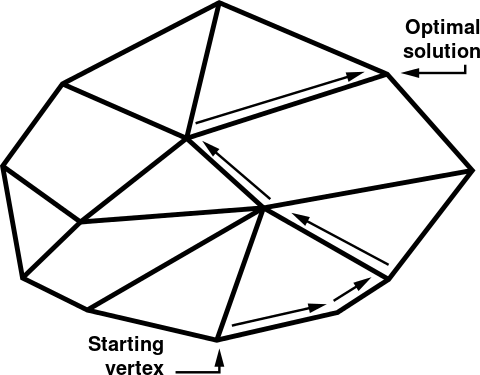
\includegraphics[width=0.4\textwidth]{simplex-graphically}
        \caption{Representación gráfica del modo de ejecución del algoritmo \emph{Simplex}.}
        \label{img:solving_simplex}
      \end{figure}

      \paragraph{}
      Hasta ahora, en este apartado se ha descrito únicamente el proceso de resolución mediante algunos métodos exactos. Sin embargo, no se ha realizado ninguna particularización sobre el problema \emph{Dial-a-Ride}. Por tanto, es momento de definir el punto de enlace entre la definición del método y el problema en cuestión. Tal y como se ha descrito a lo largo del \cref{chap:formulation} el problema \emph{Dial-a-Ride} se enmarca dentro de los problemas de \emph{optimización lineal}. En la \cref{eq:formulation_basic_darp} se describe la formulación de $3$ índices para este problema, incluyendo tanto las variables de decisión como las restricciones que lo componen. En cuanto a la estrategia de enumeración, es fácil darse cuenta de que esta puede llevarse a cabo tomando todas las combinaciones posibles para las variables binarias del problema (lo cual tal y como se ha comentado anteriormente es algo inabordable en problemas no demostrativos). En cuanto a la estrategia de resolución basada en el algoritmo \emph{Simplex}, tal y como se ilustra en \cite{klee1970good} es posible construir la matriz simplex a partir de la matriz de restricciones generada por el problema en forma lineal.

      \paragraph{}
      A lo largo de la literatura relacionada con métodos de resolución exactos para el problema \emph{Dial-a-Ride}, existen un gran número de referencias basadas en el estudio de técnicas basadas en \emph{Branch and Bound} que tratan de tomar ventaja de alguna manera de la estructura del problema para así simplificar el camino hasta la solución óptima. En el siguiente apartado se describen de manera más detallada los conceptos en que se apoya este método.

      \subsection{Branch and Bound}
      \label{sec:solving_branch_bound}

        \paragraph{}
        Se pueden englobar en la categoría de algoritmos \emph{Branch and Bound} todos aquellos que basan su estrategia de resolución en comenzar por una versión relajada del problema base para posteriormente realizar un proceso jerarquico de cambios sobre la estructura del problema hasta alcanzar el valor óptimo del mismo. Esta estrategia es muy usada sobre problemas de \emph{optimización entera} ya que facilita en gran medida la problemática generada por las variables de decisión de carácter discreto del problema.

        \paragraph{}
        La estrategia habitual consiste en partir de una versión del problema sobre la cual las restricciones sobre variables discretas se han relajado a valores sobre intervalos. Es decir, supongamos que la variable de decisión $x$ únicamente puede tomar valores enteros entre $1$ y $5$, lo que es equivalente a $x \in \{1,2,3,4,5\}$. Entonces, una relajación lineal podría venir dada por la transformación en $1 \leq x \leq 5$ la cual es más sencilla de resolver por el algoritmo \emph{Simplex}. Posteriormente, el resto de pasos de ramificación consisten en añadir restriciones (mediante la generación de filas o columnas) que permitan satisfacer las restricciones del problema original.

        \begin{figure}[ht]
          \centering
          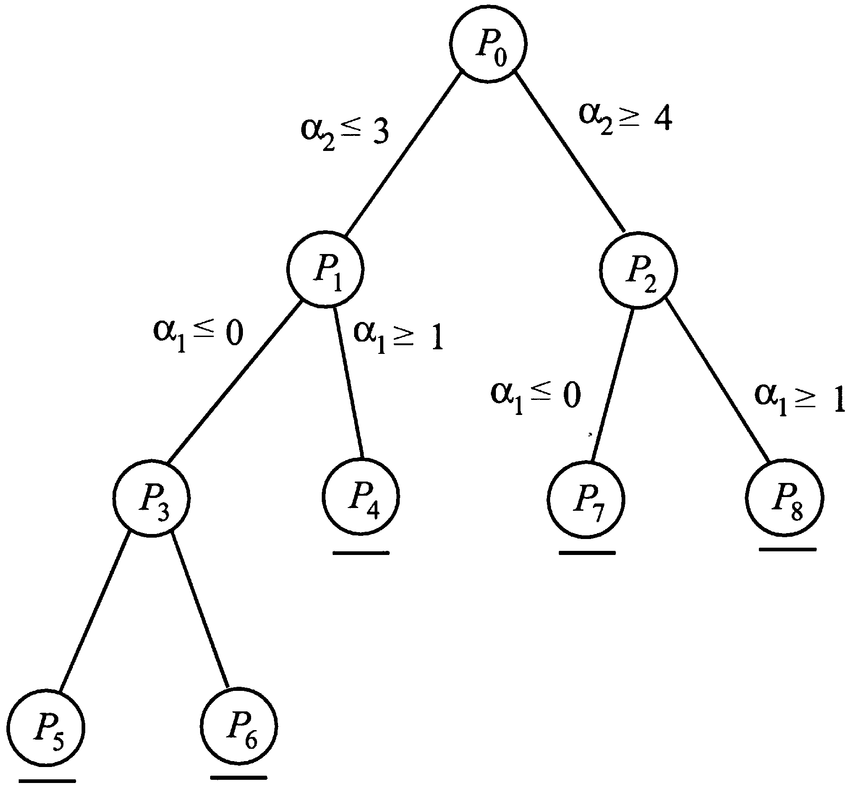
\includegraphics[width=0.4\textwidth]{branch-and-bound-tree}
          \caption{Ejemplo de ramificación del problema mediante el algoritmo \emph{Branch and Bound}.}
          \label{img:branch_and_bound}
        \end{figure}

        \paragraph{}
        Es importante tener en cuenta que las relajaciones aplicadas al problema inicial para aplicar el algoritmo \emph{Branch and Bound} no tienen por qué ser de naturaleza lineal, si no que se pueden aplicar sobre otros tipos de restricciones. Un ejemplo de ello se podría dar eliminando por ejemplo las restricciones de duración máximo de viaje en el problema \emph{Dial-a-Ride}, o la eliminación de restrcciones de ventana temporal en el problema \emph{Pickup and Delivery with Time Windows}. Una vez generada una solución factible sobre estos casos, el proceso de ramificación consistirá en \say{modificar} dicha solución hasta alcanzar aquella que cumpla todas las restricciones (de tiempo máximo de viaje, de ventanas temporales, etc.).

        \paragraph{}
        Dependiendo de la estrategia de ramificación del algoritmo, este se denomina de distintas maneras. Cuando la ramificación se basa en la generación de filas el algorimo se conoce como \emph{Branch and Cut}, mientras que si la estrategia se basa en la generación de columnas este se denomina \emph{Branch and Price}. Por último, cuando la estrategia se basa en la combinación de ambos entonces el algorimo es denominado \emph{Branch and Cut and Price}.

        \subsubsection{Branch and Cut}
        \label{sec:solving_branch_cut}

          \paragraph{}
          Tal y como se ha comentado anteriormente, los algoritmos \emph{Branch and Cut} consisten en una caracterización del algoritmo general de ramificación donde el proceso de \say{estrechamiento} de la versión relajada para cumplir con todas las restricciones impuestas por el problema viene dado por la adicción de planos de corte a partir de nuevas restricciones. Es por ello que este método se apoya en estrategias de generación de filas.

          \paragraph{}
          Para el caso del problema \emph{Dial-a-Ride}, en \cite{cordeau2006branch} se propone una implementación completa basada en el algoritmo \emph{Branch and Cut} la cual se apoya en la generación inicial de una solución del problema relajado (para el cual se eliminan las restricciones que imponen variables de decisión binarias, permitiendo que estas tomen cualquier valor en el intervalo $[0, 1]$) para posteriormente, a partir de un proceso de ramificación añadir restricciones adiccionales que fuerzan a las variables de naturaleza binaria con valores no binarios a tomar un valor válido (ahí surge el proceso de ramificación). Para detectar sobre qué variable concreta generar el corte en cada caso, la estrategia seguida se apoya en la definición de unas heurísticas que generan una lista ordenada sobre la cual seleccionar dicha variable. En la línea de este enfoque, también es interesante remarcar \cite{ropke2007models} donde además se propone un modelo de optimización combinatoria basado en 2 índices, que a pesar de no representar el mismo caso que el problema \emph{Dial-a-Ride}, sus diferencias son mínimas (número indeterminado de vehículos, todos los vehículos con misma capacidad, etc.).

        \subsubsection{Branch and Price}
        \label{sec:solving_branch_price}

          \paragraph{}
          Del mismo modo que el método \emph{Branch and Cut} es una estrategia de generación de filas enmarcada dentro de la familia de algoritmos \emph{Branch and Bound}, el método \emph{Branch and Price} es la versión correspondiente cuya estrategia se basa en la generación de columnas sobre la matriz de restricciones del problema de programación lineal. Es decir, se basa en la inclusión de nuevas variables sobre una versión relajada del problema inicial. Puesto que puede dar lugar a confusión, es necesario detallar cómo se puede llevar esto a cabo para reflejar de manera adecuada la diferencia respecto del método de generación de filas. Mientras que en la estrategia de generación de filas, la relajación se produce permitiendo que las variables de decisión tomen valores que no satisfacen las restricciones originales, en este caso el enfoque consiste en resolver una versión más simple del problema original para después, mediante un proceso iterativo, ampliar el alcance del problema simplificado hasta alcanzar la definición del mismo que satisfaga todas las restricciones de la versión original. El proceso de ramificación surge cuando no es posible satisfacer las condiciones impuestas tras la inclusión de nuevas variables, donde esta es forzada con la esperanza de que sea satisfecha en la siguiente iteración, creando una ramificación por cada posible alternativa.

          \paragraph{}
          Aplicado al problema \emph{Dial-a-Ride}, una posible estrategia se apoya en limitar los aristas disponibles del grafo en una primera iteración, para posteriormente aplicar un proceso inclusión/eliminación de aristas del grafo para así controlar la complejidad del problema a la vez que se exploran distintas soluciones. El proceso de ramificación de soluciones surge cuando son eliminados aristas que en alguna de las soluciones hayan sido utilizados. Para llevar a cambo dicho proceso de inclusión/eliminación en la literatura se han propuesto estragias apoyadas en \emph{Programación dinámica}.

        \subsubsection{Branch and Cut and Price}
        \label{sec:solving_branch_cut_price}

          \paragraph{}
          Una vez descritos lo métodos basados en generación de filas (\emph{Branch and Cut}) así como de columnas (\emph{Branch and Price}), es fácil entender el funcionamiento del método \emph{Branch and Cut and Price}, que se apoya en la combinación de ambas estrategias para reducir así reducir la complejidad de resolución del problema \emph{Dial-a-Ride}. Como es natural, estos cuentan con la ventaja de resolver instancias más fáciles de resolver del problema por tener un menor número de restricciones (eliminación de filas) así como de hacerlo sobre versiones más pequeñas del problema (eliminación de columnas). Tal y como se ha podido comprobar en distintas publicaciones que comparan la utilización de los métodos de generación de filas o columnas de manera separada, frente a las correspondientes versiones combinadas, estas últimas obtienen un nivel de resultados equivalente requiriendo de un menor nivel de cómputo.

      \paragraph{}
      Tal y como se ha podido comprobar a lo largo del apartado, los métodos de resolución apoyados por técnicas basadas en ramificación son capaces de ofrecer ventajas relacionadas con la simplicación del problema completo a resolver a costa de requerir la resolución de múltiples versiones relajadas de distintas formas de dicho problema. Cuando el tamaño de la instancia del problema es tan grande que esta no puede ser resuelta \say{de una sola vez}, estos métodos ofrecen una alternativa interesante por seguir ofreciendo garantías de optimalidad, lo cual en ciertos casos es un requisito necesario.

    \section{Métodos de Resolución basados en Heurísticas}
    \label{sec:solving_heuristics}

      \paragraph{}
      Tal y como se ha explicado anteriormente, los problemas de optimización combinatoria se corresponden en la mayoría de ocasiones con problemas cuya complejidad desde el punto de vista de la resolución no es sencilla. Tal es así que muchos de estos se engloban dentro de la categoría de problemas $NP$, lo cual se puede resumir como aquellos para los cuales no existe una estrategia de resolución exacta que alcance el resultado óptimo en tiempo polinómico. Esto implica que para instancias no demasiado grandes no sea factible alcanzar dicho resultado en un tiempo aceptable.

      \paragraph{}
      Para paliar esta problemática, surgen métodos de resolución denominados \emph{estrategias heurísticas}. Estas se caracterizan por ser capaces de proporcionar resultados razonablemente cercanos a solución óptima empleando para ello una cantidad de recursos (generalmente tiempo de cómputo) significativamente menor a la que requerirían otras estrategias con ganarantías de optimalidad. Este es un compromiso aceptable cuando no es posible llegar a soluciones de otro modo. Por lo tanto, uno de los grandes objetivos de la investigación y el desarrollo de heurísticas consiste en implementar algoritmos que sean capaces de alcanzar soluciones lo más cercanas a la solución óptima, teniendo en cuenta las restricciones de tiempo para que estas puedan ser alcanzadas.

      \paragraph{}
      Desde una perspectiva de alto nivel, los métodos de resolución basados en heurísticas típicamente son clasificados en dos grandes categorías según la función que desempeñan, las cuales se conocen como \emph{heurísticas de construcción} y \emph{heurística de mejora}. A pesar de que su nombre es lo suficientemente explicativo, a continuación se detalla la función que representan los métodos pertenecientes a cada una de estas categorías:

      \begin{itemize}

          \item \textbf{Heurísticas de Construcción}: la función que desempeñan consiste en la generación de soluciones sin el apoyo de ningún estado previo. Es decir, recibiendo únicamente los valores de entrada necesarios para la formulación del problema, estas son capaces de generar soluciones del problema que satisfacen todas las restricciones impuestas por la formulación del mismo. En el caso de los problemas de rutas de vehículos, estas estrategias se apoyan comúnmente en algorimos de inserción inspirados en algoritmos greedy y, en algunas ocasiones con un cierto nivel de aleatoriedad. Por lo general, los resultados a los que es posible llegar utilizando únicamente estrategias de este tipo, no son lo suficientemente cercanas al resultado óptimo. Para resolver esta problemática, existen otras estrategias que tratan de paliar esta situación.

          \item \textbf{Heurísticas de Mejora}: debido al grado de dificultad necesario para tomar las decisiones más acertadas durante el proceso de construcción de soluciones, la categoría de \emph{heurísticas de mejora} trata de mejorar la calidad una solución dada. Para ello, como es esperable, estas estrategias necesitan conocer tanto el conjunto de valores de entrada necesarios para la formulación del problema, como una solución inicial del mismo. A partir de estas dos partes, el modo de funcionamiento consiste en aplicar distintas modificaciones a la solución para así tratar de maximizar (o minimizar) el valor de la función objetivo, lo cual acerca dicha solución al valor óptimo deseado. A este modo de funcionamiento se le conoce como búsqueda local dentro del espacio de soluciones. En el caso de los problemas de rutas de vehículos, las estrategias en que se basan consisten en la aplicación de operadores tales como el intecambio de tareas (o viajes) entre distintos vehículos, cambio del orden dentro del mismo vehículo, etc. Por tanto, el objetivo se trata de buscar el conjunto de transformaciones de la solución que permitan un mayor acercamiento al resultado esperado al final de la ejecución. Esta última afirmación se explicará más en detalle en el \cref{sec:solving_greedy}

      \end{itemize}

      \paragraph{}
      Una vez se han detallado las diferencias entre las dos categorías principales de estrategias de resolución basados en heurísticas, se está en condiciones suficientes como para explicar en detalle algunos de los algoritmos concretos a través de los cuales es posible alcanzar dichas soluciones. El resto del apartado se estructura de la siguiente forma: en el \cref{sec:solving_brute_force} se detalla la estrategia basada en \emph{fuerza bruta} (la cual como veremos no es aplicable en la práctica en la gran mayoría de casos). Seguidamente, en el \cref{sec:solving_random} está dedicado a la estrategia basada en \emph{selección aleatoria}. Después se describirá en detalle la estrategia basada en \emph{algoritmos greedy} (la cual es muy popular por su sencillez conceptual y relativamente buenos resultados). Posteriormente se discutirá el funcionamiento de la estrategia de \emph{clarke and wright} y un método basado en \emph{redes neuronales} en los \cref{sec:solving_clarke_and_wright,sec:solving_neural_networks}. Finalmente, se describirá la categoría de heurísticas conocidas como de \emph{Búsqueda Local}, las cuales presentan una naturaleza diferente tal y como se comenta en el apartado correspondiente.

      \subsection{Fuerza Bruta}
      \label{sec:solving_brute_force}

        \paragraph{}
        A pesar de que anteriormente se ha comentado que una de las grandes diferencias entre métodos de resolución exactos y métodos de resolución basados en heurísticas son las garantías de optimalidad, esta distinción es un tanto difusa cuando se tratan de clasificar las estrategias de fuerza bruta. Esto se debe a que, si bien es cierto que esta estrategia es capaz de garantizar resultados óptimos cuando termina, la estrategia de resolución se encuentra más próxima a los algoritmos heurísticos que a los métodos que hemos clasificado como exactos, puesto que estos se apoyan en mayor medida en la teoría de programación lineal mixta, mientras que las estrategias heurísticas tienden a acercarse más a estrategias algorítmicas clásicas. Para una descripción más detallada y profunda del tema se recomienda consultar \cite{cormen2009introduction}.

        \paragraph{}
        Una vez aclarada la peculiaridad de la estrategia de \emph{fuerza bruta}, procedemos a describir en qué se basa: El modo de funcionamiento consiste en la enumeración de todas las posibles configuraciones, para después proceder a filtrar todas aquellas que sean factibles, y de entre estas, escoger aquella que maximize (o minimize) la función objetivo. La definición de esta estrategia en pseudo código se incluye en el \cref{code:solving_brute_force} (donde $U$ representa el universo de posibles soluciones, $feasible$ se trata de una función que recibe una solución y se encarga de evaluar si es o no factible, $F$ se compone de todas las soluciones factibles y por último, $s$ se corresponde con la solución óptima, que en este caso se trata de un problema de minimización).

        \begin{algorithm}[ht]
          \SetAlgoLined
          \KwResult{$s$ }
          $F \gets filter(feasible, U)$\;
          $s \gets min\{F\}$\;
          \caption{Estrategia de resolución basada en \emph{fuerza bruta}.}
          \label{code:solving_brute_force}
        \end{algorithm}

        \paragraph{}
        Sin embargo, tal y como se puede intuir, esta estrategia de resolución requiere de una cantidad de recursos que crece de manera exponencial respecto del tamaño de entrada. Por lo tanto, no es aplicable en la práctica sobre problemas de gran tamaño. Aún así, existen ciertos problemas para los cuales el grado de complejidad es relativamente bajo o el tamaño de las instancias a resolver es pequeño, por lo que esta estrategia es aplicable. En dichos casos, esta es una alternativa interesante ya que, como se ha comentado anteriormente, los algoritmos basados en \emph{fuerza bruta} proporcionan garantías de optimalidad.

        \paragraph{}
        Una de las ventajas de los métodos de resolución basado en fuerza bruta es la capacidad de poder aprovecharse de la estructura del problema concreto que se pretende resolver para así poder reducir el espacio de búsqueda de soluciones en gran medida. Esto se debe a que el espacio de posibles soluciones factibles es un subconjunto del espacio de posibles soluciones. Por tanto, si se consigue encontrar alguna estrategia que permita enfocarse únicamente en las soluciones factibles, los requerimientos computacionales serán mucho menores. Un ejemplo de ello podría aplicarse a una estrategia de generación de soluciones en problemas de rutas a partir de una estrategia de inserción al final de la ruta. Entonces, es fácil darse cuenta de que si durante el proceso de inserción de tareas en la ruta, se llega a un estado de infactibilidad, continuar el proceso de insertar nuevas tareas al final de la ruta, continuará generando soluciones infactibles. Por tanto, en este caso es posible reducir el espacio de búsqueda sin perder las garantías de optimalidad.

      \subsection{Selección Aleatoria}
      \label{sec:solving_random}

        \paragraph{}
        La siguiente estrategia heurística a comentar se presenta en muchos sentidos como una versión opuesta a la de \emph{fuerza bruta}. Esta es la heurística basada en \emph{selección aleatoria}, cuya principal característica es el apoyo en una componente de estocasticidad que pretende, a largo plazo, alcanzar resultados razonables utilizando para ello un reducido coste computacional. Entonces, tal y como se puede intuir esta estrategia es opuesta a la de \emph{fuerza bruta} en dos sentidos: \begin{enumerate*}[label=(\arabic*)] \item la búsqueda en el espacio de soluciones no es exhaustiva, por lo que no se prueban todos los casos posibles (lo cual elimina las garantías de optimalidad) y \item el coste computacional que conlleva generar soluciones factibles es mucho menor puesto que la decisión sobre qué camino explorar se delega en selección aleatoria \end{enumerate*}.

        \paragraph{}
        Tal y como se puede apreciar en el \cref{code:solving_random_selection}, la estrategia se basa en generar soluciones aleatorias del universo de posibles soluciones para después evaluar la factibilidad de la escogida en cada iteración y almacenarla en caso de que esta maximice (o minimice) el valor de la función objetivo. Esto se repite mientras se cumpla una determinada condición, la cual puede basarse en un determinado número de iteraciones, una cantidad de tiempo o estrategias más elaboradas como un ratio de mejora respecto entre la última mejor solución obtenida y la anterior, etc.

        \begin{algorithm}[ht]
          \SetAlgoLined
          \KwResult{$s$ }
          $s \gets \emptyset$\;
          \While{$condition$}{
              $c \gets random(U)$\;
              \If{$!feasible(c)$}{
                  \Continue\;
              }
              $s \gets min(s, c)$\;
          }
          \caption{Estrategia de resolución basada en \emph{selección aleatoria}.}
          \label{code:solving_random_selection}
        \end{algorithm}

        \paragraph{}
        Tal y como se puede intuir, por si sola esta heurística no es todo lo eficiente como se espera para ser aplicable en la práctica puesto que, a pesar de la simplicidad que proporciona durante el proceso de generación y evaluación de soluciones, resulta muy improbable que llegue a alcanzar soluciones razonables sin que la estrategia se apoye en cierto conocimiento del problema. Sin embargo, tal y como se comentará más adelante, esta estrategia sirve como base (o componente) de otras mucho más elaboradas que consiguen alcanzar resultados mucho mejores en el largo plazo mediante la utilización de cierta componente aleatoria en alguna parte del proceso de optimización. Desde el punto de vista conceptual, hacer esto consigue añadir cierto ruido en el camino de búsqueda hacia la solución óptima que puede ser positivo dado que este reduce la complicación de \say{caer} en máximos (o mínimos) locales que en ciertas estrategias heurísticas complican en gran medida el proceso de optimización.

      \subsection{Greedy}
      \label{sec:solving_greedy}

        \paragraph{}
        Una de las estrategias más conocidas (por su buena relación entre sencillez y calidad de las soluciones) son las basadas en \emph{algorithmos greedy}. Estos se corresponden con una de las principales categorías en las cuales se suelen dividir los algoritmos en la mayoría de libros de relacionados. La principal característica de este tipo de algoritmos es que cada una de las decisiones que toman se convierten en invariantes para los próximos pasos que lleve a cabo la estrategia en la búsqueda de la solución final. De ahí el nombre \emph{greedy} (o voraz en español), que trata de remarcar la idea de que cada una de las decisiones que tomadas terminarán formando parte de la solución final. Nótese que esta condición conlleva dos consecuencias principales \begin{enumerate*}[label=(\arabic*)] \item la simplicidad tanto a nivel conceptual como conceptual al requerir únicamente del estado actual (obtenido a partir de las decisiones tomadas anteriormente y las alternativas actualmente posibles), y \item la restricción de reevaluar decisiones anteriores que permitirían llegar a una solución más acercada con el conocimiento obtenido en el momento actual \end{enumerate*}.

        \paragraph{}
        Sin embargo, existen ciertos problemas que poseen ciertas características que permiten que los algoritmos de naturaleza voraz sean capaces de llegar al resultado correcto (u óptimo dependiendo de la naturaleza del problema) de manera eficiente y a la vez sencilla. El ejemplo más notable es el de el \emph{problema del cajero}. Dicho problema consiste en la elección sobre qué monedas utilizar de entre un conjunto dado de posibles valores (los cuales no tienen restricciones de cardinalidad) de tal manera que el número de monedas que sea mínimo. A modo de ejemplo, suponiendo el conjunto de valores posibles $\{1,5,10, 25, 100\}$, la asignación que minimiza el número de monedas para devolver el valor $34$ es de $[25, 5, 1, 1, 1, 1]$. La estrategia para llegar a esta solución consiste en seleccionar siempre la moneda de mayor valor que no supere el resto necesario para llegar al valor deseado. En el \cref{code:solving_greedy} se muestra el pseudo código de la estrategia, donde $S$ representa la solución, $v$ el valor deseado, $C$ el conjunto de posibles monedas y $c$ una variable temporal. Tal y como se puede apreciar, siguiendo esta estrategia se cumplen las condiciones requeridas po los \emph{algoritmos de naturaleza voraz} ya que únicamente se tiene en cuenta el estado actual para tomar la siguiente decisión y no se modifican las decisiones tomadas anteriormente. Para más información acerca de las características de esta categoría algorítmica así como ejemplos más interesantes se recomienda consultar \cite{cormen2009introduction}.

        \begin{algorithm}[ht]
          \SetAlgoLined
          \KwResult{$S$ }
          $S \gets [] $\;
          \While{$v \neq 0$}{
            $c \gets min_{v - c > 0}\{C\}$\;
            $v \gets v - c $\;
            $S \gets S + [ c ]$\;
          }
          \caption{Estrategia de resolución del \emph{problema del cajero} basada en \emph{algoritmo greedy}.}
          \label{code:solving_greedy}
        \end{algorithm}

        \paragraph{}
        Desde el punto de vista de los problemas de optimización combinatoria, los \emph{algoritmos de naturaleza voraz} han sido de gran utilidad para muchas situaciones. Sin embargo, tal y como se puede intuir, estos requieren que el problema sobre el que se van a aplicar cumpla la propiedad de ser concavos (una mejora sobre una solución arbitraria en la dirección de la solución óptima garantiza un menor coste en la función objetivo) para que estos puedan alcanzar la solución óptima. Por contra, esto ocurre en muy pocas ocasiones en la mayoría de problemas de optimización combinatoria. Si bien es cierto, hay casos para los cuales esta condición si se cumple (como el problema del cajero), pero en muchos otros (entre los que se encuentran los \emph{problemas de rutas de vehículos}) esta condición no se satisface.

        \paragraph{}
        A pesar de ello, tal y como se ha indicado anteriormente, estos algoritmos son capaces de proporcionar resultados relativamente razonables utilizando una cantidad de recursos muy contenida por lo que cuando es tolerable cierto nivel de error respecto de la solución óptima, como es el caso cuando se recurre a estrategias basadas en heurísticas, estos algoritmos proporcionan resultados muy interesantes. Como es natural, el modo en que estos se aplican es muy dependiente de la naturaleza del problema en cuestión. Sin embargo, en el ámbito de los \emph{problemas de optimización combinatoria} es común que la estructura de los mismos tenga unas cierta forma: \textbf{Por lo general, los algoritmos greedy se construyen como un bucle condicional donde se controlan cuestiones relacionadas con el alcanzamiento de una solución final, ya sea debido a la falta de recursos u otros motivos. La acción que se repite en el bucle típicamente es la selección de la mejor alternativa de entre un conjunto de posibles opciones que modifican tanto el valor de la función de coste como el estado actual de una determinada manera.}

        \paragraph{}
        Entonces, un factor decisivo a la hora de aplicar \emph{algoritmos de naturaleza voraz} se basa en elegir de manera adecuada el criterio de selección que se utilizará para elegir la siguiente alternativa que aplicar tras cada iteración del bucle condicional. En el siguiente apartado se describen algunos de los más utilizados en los problemas de optimización combinatoria.

        \subsubsection{Criterios de Selección}
        \label{sec:solving_greedy_criterions}

          \paragraph{}
          Los criterios de selección en las heurísticas basadas en \emph{algoritmos de naturaleza greedy} representa una de las decisiones más importantes durante el proceso de configuración de este tipo de estrategias dado que son las causantes de priorizar la toma de unas decisiones frente a otras. Como es natural, dichos criterios de selección son muy dependientes de la naturaleza del problema a resolver. Los problemas relacionados con el aprovisionamiento de recursos tienen por tanto criterios de selección muy diferentes a otros como los relacionados con la generación de rutas de vehículos.

          \paragraph{}
          Dado que el trabajo se enfoca en el problema \emph{Dial-a-Ride}, a continuación se comentan algunos de los criterios de selección más comunes para este tipo de problemas:

          \begin{itemize}

            \item \textbf{Ruta con menor duración}: Se trata de seleccionar siempre la alternativa que genera la ruta con menor duración. Esta tiende a generar soluciones con rutas de duraciones similares (cuando todos los vehículos disponen de la misma cantidad de tiempo de duración y las visitas se distribuyen de manera uniforme).

            \item \textbf{Parada más cercana}: Se trata de seleccionar la alternativa con menor distancia a la ruta en cuestión. De esta forma se tiende a reducir la distancia global de las rutas, lo cual tiende a reducir el coste pero a su vez es propicio a caer mínimos locales.

            \item \textbf{Fin de ventana temporal más temprana}: Prioriza aquellos viajes que mayor riesgo tienen de no ser satisfechos debido a su ventana temporal respecto del estado del vehículo.

            \item \textbf{Viaje más corto}: Se trata de seleccionar primero aquellos viajes que generan el tiempo de viaje más corto (teniendo en cuenta las posibles paradas intermedias). A pesar de que esta estrategia tiende a reducir el tiempo global, también tiende a aumentar el coste de la ruta dado que en muchas situaciones añadir paradas intermedia genera reducciones drásticas.

          \end{itemize}

          \paragraph{}
          Elegir de manera adecuada el criterio de selección que mejor se ajusta a las características concretas del problema a resolver, y de las situaciones que se generan en las instancias a resolver es un factor a tener en cuenta. Sin embargo, en este tipo de problemas la resolución óptima de las soluciones parciales no mantiene una correlación perfecta con la resolución óptima de la solución global.

          \paragraph{}
          Es por ello que existen ciertas técnicas que tratan de paliar dichas dificultades, entre las que se encuentran métodos adaptativos, que conforme evoluciona la ejecuión generan ciertas variaciones en los criterios de selección, u otras basadas en la aleatorización controlada como \emph{Randomized Greedy} que se comenta a continuación.

        \subsubsection{Randomized Greedy}
        \label{sec:solving_randomized_greedy}

          \paragraph{}
          A pesar de que la elección de un criterio de selección adecuado para el problema que se pretende resolver, existen ocasiones en que estos no son lo suficientemente \say{buenos} como se podría esperar. Por la propia naturaleza de los algoritmos de naturaleza voraz, en muchas ocasiones no es suficiente el contexto actual para escoger la decisión más acertada a largo plazo.

          \paragraph{}
          Para tratar de suavizar el peso de dicha decisión uno de los enfoques posibles es el de añadir un cierto grado de aleatoriedad en el momento de elegir el la mejor opción a realizar. Es decir, en lugar de seguir una estrategia que escoja siempre el la opción que maximize (o minimice) el valor del criterio de selección, se escoge aleatoriamente la siguiente opción de entre las mejores posibles. Como se ha comentado, la idea subyacente tras esta estrategia es que se asume que el criterio de selección escogido, a pesar de ser óptimo en el momento de su utilización (resultado parcial), probablemente no lo sea respecto del resultado completo. Entonces, la componente aleatoria trata de reducir dicho efecto generado por las \say{malas decisiones} tomadas.

          \paragraph{}
          Generalmente, para llevar a cabo la selección aleatoria se mantiene una lista ordenada con las $k$ mejores opciones posibles (de acuerdo con el criterio de selección) para después utilizar algun generador aleatorio de valores de una distribución aleatoria discreta que finalmente eligen la alternativa que finalmente utilizar. Estas distribuciones pueden ser de distinta naturaleza, aunque las más comunes son la la distribución uniforme discreta o alguna distribución armónica decreciente respecto del orden obtenido por el criterio de selección.

          \paragraph{}
          Como es esperable, estas estrategias tienden a mejorar los resultados obtenidos por los métodos greedy simples en promedio, pero obtienen peores resultado en el peor caso. Por lo tanto, su uso está muy extendido en metaheurísticas basadas en la generación de muchas soluciones. En concreto, este método se utiliza por las metaheurísticas \emph{GRASP} tal y como se comentará en el \cref{sec:solving_grasp}.

      \subsection{Clarke and Wright}
      \label{sec:solving_clarke_and_wright}

        \paragraph{}
        Una de las estrategias heurísticas más conocidas para los problemas de optimización de rutas (y que es también aplicable al problema \emph{Dial-a-Ride}) es la de ahorros (\emph{Savings}) definida por Clarke y Wright en \cite{clarke1964scheduling}. La estrategia esta definida asumiendo que no existen limitaciones en cuanto al número de vehículos disponibles para resolver el problema, por lo que esto es algo a tener en cuenta para su utilización. Sin embargo, es posible realizar pequeñas modificaciones que permitan su utilización con restricciones del número de vehículos. Una manera trivial de hacer esto es la de eliminar tantas rutas como sea necesario hasta que se cumplan las restricciones del número de vehículos sobre la solución generada por la heurísticas, aunque también se pueden aplicar otros enfoques como una penalización de costes elevada que limite el uso de más vehículos.

        \paragraph{}
        En cuanto al modo de funcionamiento de esta heurística, en un paso inicial genera una ruta desde almacen a cada tarea (en el caso del problema \emph{Dial-a-Ride} esto consistirá en las dos paradas que requiere el viaje, la de recogida y la de entrega). Esto hace que sean en una situación inicial sean necesarios tantos vehículos como tareas a satisfacer. Posteriormente, se lleva a cabo un proceso iterativo de fusión de rutas mientras los costes de estas sean reducidos. Es decir, se calculan el coste total que genera cada par de rutas de manera independiente para posteriormente compararlo con el coste obtenido de combinar ambas rutas. En cada ciclo del algoritmo se escoge la opción que minimiza los costes y esta exploración se repite hasta que no haya opciones de mejora posibles. Es interesante remarcar que las estrategias de combinación de rutas no están limitados a la concatenación, sino que la estrategia se basa en la valoración de todos los posibles puntos en que una ruta se puede incluir en la otra. Esto hace que sea una estrategia de muy exhaustiva en el sentido de ser capaz de probar muchas situaciones.

        \paragraph{}
        Sin embargo, el motivo de la popularidad que ha recibido esta heurística durante tanto tiempo no solo se debe al método en si, sino a que además en \cite{clarke1964scheduling} se describe la manera en que poder calcular el nivel de ahorro (de ahí el nombre de la estrategia) de la combinación de dos rutas sin tener que calcularlo los costes completos de ambas rutas y después hacer la diferencia respecto de la versión combinada. La estrategia en que se apoyan para llevar esto a cabo es la diferencia entre los costes de los tramos de inicio y fin de la ruta que se va a insertar frente a los costes de los tramos de unión entre ambas rutas. Nótese que esta estrategia es altamente eficiente cuando las tareas tienen restricciones muy flexibles tanto desde el punto de vista de las ventanas temporales como de la capacidad del vehículo. En problemas más complejos como el \emph{Dial-a-Ride} estas mejoras han de ser tomadas con prudencia ya que es necesario verificar la factibilidad de la ruta resultante.

      \subsection{Redes Neuronales}
      \label{sec:solving_neural_networks}

        \paragraph{}
        En los últimos años, el aumento de la capacidad computacional (sobre todo aplicable a operaciones de naturaleza matricial apoyado en gran parte por la evolución de las \emph{unidades de computación gráficas (GPUs)}) a propiciado un incremento exponencial la cantidad de aplicaciones reales basadas en técnicas basadas en redes neuronales (cuyos requerimientos computacionales encajan perfectamente en dicho marco). Además de las aplicaciones prácticas, también ha surgido un gran incremento desde el punto de vista de la cantidad de artículos científicos relacionados con la materia. Entre otros temas, uno de los contextos en que se ha tratado de estudiar la factibilidad de este tipo de técnicas han sido los problemas de optimización combinatoria. Algunos de los más destacados son \cite{potvin1993state,ghaziri2003neural,leung2004expanding,masutti2009self,bello2016neural}. Tal y como se puede apreciar, estos trabajos tienen en común la utilización de enfoques basados en \emph{redes neuronales recurrentes} así como \emph{mapas auto-organizados}. A continuación se describen brevemente este tipo de arquitecturas:

        \begin{enumerate}

            \item \textbf{Redes Neuronales Recurrentes}: Consisten en una clase de redes neuronales con la característica de utilizar los pesos de ciertas neuronas de las capas internas como valores de entrada, creando una relación de recurrencia con la que se espera obtener la capacidad de tener un estado interno en la red. Es por ello que su utilización en el campo del análisis de lenguaje natural es muy interesante.

            \item \textbf{Mapas Auto-Organizados}: Se trata de una arquitectura de red neuronal que se caracteriza por tener en cuenta la localización de las neuronas para el entrenamiento de la misma (que se organizan en forma de rejilla). Esto implica que los pesos de estas estén basados en la posición de las mismas. Es por ello que se su utilización en procesos de visualización de datos utilizados en tareas de clustering es muy interesante.

        \end{enumerate}

        \paragraph{}
        Tras haber descrito brevemente estas dos arquitecturas de redes neuronales es fácil darse cuenta de las ideas en las que se apoyan los artículos anteriormente citados. En el caso de las técnicas basadas en redes neuronales recurrentes se espera \say{descubrir} un patrón de resolción común inherente a un problema de rutas concreto y no visible de manera natural, que las capacidades recurrentes de la red sean capaz de captar. En el caso de las técnicas basadas en mapas auto-organizados, la idea es que (por la estructura en forma de mapa de la red) se descubran patrones de cercanía entre las distintas localizaciones a visitar durante la ruta, con las que después se puedan reconstruir caminos de coste reducido.

        \paragraph{}
        Dichas estrategias presentan un gran potencial sobre aquellos problemas que presenten las características comentadas anteriormente. Sin embargo, hasta la fecha dichas ideas se encuentran todavía en fases muy tempranas de investigación por lo que no son aplicables en situaciones reales (en \cite{bello2016neural} fueron necesarias 7 horas de computación para resolver una instancia del problema del viajero de $50$ localizaciones). Sin embargo, si que forman parte de un interesante nicho de investigación que podría ser muy prometedor en el futuro.

      \subsection{Búsqueda Local}
      \label{sec:solving_local_search}

        \paragraph{}
        [TODO]

      \paragraph{}
      En este apartado se han descrito las principales estrategias heurísticas utilizadas en problemas de optimización de rutas, las cuales sirven de base para resolver las características concretas que se presentan en el problema \emph{Dial-a-Ride}. Tal y como se comentó al principio del mismo, estas estrategias destacan por su relativa sencillez, tanto conceptual como computacional. Sin embargo, en muchas ocasiones no proporcionan resultados suficientemente buenos (desde el punto de vista de su distancia a la solución óptima) como se requiere. Para contrarestrar dicha situación surge una nueva clase de estrategias de optimización compuesta por otras estrategias más sencillas la cuál se discute en el próximo apartado.

    \section{Métodos de Resolución basados en Metaheurísticas}
    \label{sec:solving_metaheuristics}

      \paragraph{}
      El concepto de \emph{metaheurística} surge tras la necesidad de desarrollar estrategias de resolución apoyadas en otras (típicamente más sencillas) las cuales, en muchas ocasiones, no son capaces de proporcionar soluciones lo suficientemente satisfactorias por si solas a pesar de basarse en intuiciones coherentes para llegar a soluciones adecuadas pero que a su vez presentan alguna limitación que por si solas no les permite alcanzar el resultado deseado. En esta línea, la función de una \emph{metaheurística} trata de tener en cuenta dichas limitaciones para así tomar las decisiones pertinentes que reduzcan dichos efectos no deseados.

      \paragraph{}
      A modo de ejemplo, este tipo de acciones podría ir desde limitar la voracidad de un algoritmo greedy para evitar caer en mínimos locales, hasta controlar el tiempo de ejecución de un método de resolución exacto, cuando el ratio de mejora relativa obtenido por este alcance una determinada cota mínima. Sin embargo, las \emph{metaheurísticas} uno solo se limitan a este tipo de acciones posibles, sino que abarcan un gran número de posibilidades tal y como se verá a lo largo del apartado, la cual se orienta hacia las más populares en lo relacionado con el \emph{problema Dial-a-Ride}. En primer lugar, en el \cref{sec:solving_grasp} se describirá la estrategia \emph{GRASP}. Posteriormente, en el \cref{sec:solving_simulated_anneling} se describe la idea subyacente tras los métodos basados en \emph{Simulated Anneling}. A continuación se comenta la metaheurística de \emph{Búsqueda Tabú}. Finalmente, se comentan las metaheurísticas basadas en \emph{Busqueda de Vecindarios Variable}, \emph{Búsqueda de Gran Vecindario} en los \cref{sec:solving_vns,sec:solving_lns} respectivamente. Finalmente, se comentan brevemente las \emph{metaheurísticas basadas en poblaciones} en el \cref{sec:solving_population_metaheuristics}. Para una descripción más detallada acerca de las metaheurísticas más comunes, se recomienda consultar \cite{blum2003metaheuristics,glover2006handbook,boussaid2013survey,ho2018survey}.

      \subsection{GRASP}
      \label{sec:solving_grasp}

        \paragraph{}
        Una de las estrategias metaheurísticas más populares es la conocida como \emph{GRASP (Greedy Randomized Adaptive Search) o búsqueda adaptativa aleatorizada voraz}. Esta metaheurística es muy simple conceptualmente pero a su vez muy potente a la hora de alcanzar resultados razonables. El modo de funcionamiento se basa en lo siguiente: se repiten de manera iterativa dos operaciones principales mientras no se cumpla una determinada condición de parada. Dichas operaciones consisten en la generación de una solución inicial, posiblemente basada en una estrategia \emph{Greedy Aleatorizado}, aunque no necesariamente (existen estrategias basadas en la generación de soluciones iniciales totalmente aleatorias), y una segunda operación de mejora de dicha solución mediante una heurística de \emph{Búsqueda Local}. La condición de parada, al igual que se ha indicado en otras ocasiones, puede venir dada por un determinado número de iteraciones sin soluciones mejores u otras estrategias de naturaleza similar.

      \begin{algorithm}[ht]
        \SetAlgoLined
        \KwResult{$best$ }
        \While{$condition$}{
          $current \gets initialSolution(U)$\;
          $current \gets localSearch(current)$\;
          $best \gets min\{best, current\}$\;
        }
        \caption{Estrategia de resolución basada en metaheurística \emph{GRASP}.}
        \label{code:solving_grasp}
      \end{algorithm}

      \paragraph{}
      En el \cref{code:solving_grasp} se muestra una plantilla para la metaheurística \emph{GRASP}, la cual sigue la misma estructura que se describió en el anterior párrafo. Tal y como se ha comentado, estas estrategias gozan de gran popularidad por su sencillez y buenos resultados. Además, entre otras, presenta la ventaja de poder ser paralelizada de manera muy sencilla dado que el contenido del bucle interno es independiente tras cada etapa (obviando la parte final de comparación con la mejor solución encontrada hasta el momento). Para más información acerca de esta metaheurística se recomienda consultar \cite{resende2016optimization}, dedicado integramente a su estudio y análisis.

      \subsection{Simulated Anneling}
      \label{sec:solving_simulated_anneling}

        \paragraph{}
        Las metaheurísticas basadas en \emph{Simulated Anneling} se basan en la mejora continua de una solución inicial, siguiendo unos determinados criterios de parada (y parametrización de la etapa de búsqueda local). Esto se contrapone con la estrategia \emph{GRASP} descrita anteriormente, que se basaba en la generación de soluciones independientes para después elegir la mejor de todas ellas. En este caso, la estrategia consiste en la exploración del \emph{vecindario de soluciones} de tal manera que la opción escogida no tenga por qué ser necesariamente la que más se aproxime a la mejor solución en un primer momento, llegando al punto incluso de poder elegir ciertas opciones que empeoren el la solución actual. La idea detrás de esta estrategia se apoya en la asunción de que en fases tempranas en la etapa de busqueda de la mejor solución, decidir una opción que mueva la solución actual a un punto más lejano de la solución óptima puede ser beneficioso a largo plazo para llegar a un punto más cercano al óptimo. Dicha capacidad de \say{tomar malas decisiones} se aplica con probabilidad decreciente respecto del tiempo de ejecución actual (ya que se asume que en fases más avanzadas de la ejecución dicho comportamiento no es tan beneficioso).

        \paragraph{}
        Dicha estrategia fue desarrollada tomando como apoyo el comportamiento de ciertos metales durante su proceso de fundición, que si se lleva a cabo bajo unas determinadas condiciones de enfriamiento es posible obtener un mayor grado de resistencia. Este proceso es conocido como \emph{Simulated Anneling} (de ahí el nombre de la metaheurística). En el caso de la metaheurística, se aceptan soluciones negativas con cierta probabilidad dada por el resultado de la \cref{eq:simulated_anneling}, donde $t$ representa la temperatura (o valor decreciente respecto del número de iteraciones) y $f(s1)$ y $f(s2)$ los valores de la función objetivo para las soluciones $s1$ y $s2$ respectivamente. En el \cref{code:solving_simulated_anneling} se incluye el pseudo-código de la metaheurística.

        \begin{equation}
          \label{eq:simulated_anneling}
          P(t, f(s1), f(s2)) = exp\left(-\frac{f(s1) - f(s2)}{t}\right)
        \end{equation}

        \begin{algorithm}[ht]
          \SetAlgoLined
          \KwResult{$best$ }
          \While{$condition$}{
            \While{$annelingCondition$}{
              $current \gets randomNeighbor(best)$\;
              \If{$f(current) < f(best) \textbf{or} random(0, 1) < P(t, f(current), f(best))$}{
                $best \gets current$\;
              }
            }
            $t \gets decrease(t)$\;
          }
          \caption{Estrategia de resolución basada en metaheurística \emph{Simulated Anneling}.}
          \label{code:solving_simulated_anneling}
        \end{algorithm}

        \paragraph{}
        Esta metaheurística ha servido de base para la construcción de otras más avanzadas, como \emph{Microcanonic annealing} basado en la propiedad de equilibrio de la termodinámica, \emph{Threshold accepting method} basado en un threshold de decreciente o \emph{Noising method}. También es fácil darse cuenta de que esta metaheurística puede utilizarse de manera hibrida junto con \emph{GRASP} utilizando \emph{Simulated Anneling} como envoltorio sobre la operación de \emph{Búsqueda Local}. Las técnicas que representan el estado del arte en el área de metaheurísticas de optimización actualmente se componen principalmente de estrategias hibridas como la descrita en este caso.

      \subsection{Tabu Search}
      \label{sec:solving_tabu}

        \paragraph{}
        La metaheurística conocida como \emph{Tabu Search (o Búsqueda Tabú)} es una de las estrategias más conocidas y ampliamente utilizadas por sus buenos resultados. En concreto, en problemas de optimización de rutas existe una gran bibliografía al respecto demostrando sus buenos resultados, tanto para problemas más generales como para el \emph{Dial-a-Ride} entre los que se encuentran \cite{gendreau1994tabu,cordeau2001unified,cordeau2003tabu}.

        \paragraph{}
        La idea sobre la que se soportan las metaheurísticas basadas en \emph{Tabu Search} consiste en la utilizació de una estructura de datos de memoria que almacena la lista (restringida) de últimas soluciones visitadas para así obviarlas en próximas iteraciones y no caer en ciclos (posiblemente infinitos) de exploración de soluciones ya visitadas. Generalmente, dicha memoria está restringida a un número máximo de soluciones, que se van descartando bajo una política \emph{FIFO (First In, First Out)} lo cual incluye la posibilidad de visitar la misma solución varias veces con la esperanza de que mediante algún mecanismo aleatorio, el camino camino tomado en cada visita a la solución sea diferente. Respecto del tamaño de la memoria utilizada, el efecto que esto tiene en el proceso de optimización consiste en que memorias de menor tamaño tienden a intensificar la búsqueda sobre determinadas regiones del espacio mientras que memorias de gran tamaño tienden a realizar búsquedas más extensivas (pudiendo incluso desarrollar técnicas con memoria de tamaño variable, posiblemente decreciente).

        \begin{algorithm}[ht]
          \SetAlgoLined
          \KwResult{$current$ }
          $memory \gets \emptyset$\;
          \While{$condition$}{
              $current \gets randomNeighbor(current, ignore=memory)$\;
              $memory \gets updateMemory(memory, current)$\;
          }
          \caption{Estrategia de resolución basada en metaheurística \emph{Tabu Search}.}
          \label{code:solving_tabu_search}
        \end{algorithm}

        \paragraph{}
        En el \cref{code:solving_tabu_search} se incluye el pseudo-código que define la estructura común a las metaheurísticas basadas en búsqueda tabú. En cuanto a la intuición tras esta metaheurística, tal y como se puede apreciar, en ningún caso se restringe el movimiento hacia soluciones de \say{peor calidad} por lo que de esta manera se evita \say{caer} en mínimos locales durante el proceso de búsqueda de soluciones. Esta es una de las razones por las cuales esta metaheurística goza de tanta popularidad (sobre todo en problemas de \emph{optimización de rutas} donde el efecto dichos mínimos locales dificulta mucho el proceso). Por contra, esta metaheurística requiere de un mayor coste computacional, tanto a nivel de ejecución puesto que añade la necesidad de poder comparar si dos soluciones son o no iguales, lo cual en terminos de eficiencia no es trivial, como a nivel de espacio ya que requiere de mantener varias soluciones en memoria, lo cual es necesario tener en cuenta durante el proceso de implementación.

      \subsection{Variable Neighborhood Search}
      \label{sec:solving_vns}

        \paragraph{}
        Una de las heurísticas más interesantes en problemas de optimización de rutas es la conocida como \emph{Variable Neighborhood Search (o Búsqueda en Vecindarios Variables)} la cual se apoya en la idea de enfocar la optimización en mejorar distintos aspectos de la solución en cada fase del mismo para así terminar alcanzando una solución final de mejor calidad. Sin embargo, para poder describir esta estrategia en condiciones ideales lo primero es describir el concepto de \emph{vecindario}.

        \paragraph{}
        En el contexto de espacios de soluciones un \textbf{vecindario} consiste en un conjunto de soluciones que posseen características comunes, o que pueden ser alcanzadas aplicando operaciones similares sobre una solución inicial dada. En el caso de los problemas de optimización de rutas un vecindario puede referirse al conjunto de posibles soluciones obtenidas tras aplicar la operación de permutar dos tareas contiguas de una ruta. Entonces, este es el vecindario generado por la aplicación de dicha operación sobre una solución. Nótese que este será disjunto respecto del generado por todas las soluciones obtenidas tras aplicar la operación de permutar dos tareas no contiguas entre si. Sin embargo, esto no tiene por qué ser así, puediendo haber vecindarios que se solapan entre si.

        \paragraph{}
        Una vez entendido el concepto de \emph{vecindario}, comprender el comportamiento de esta metaheurística es muy sencillo. Se trata de seleccionar iterativamente una solución de cada vecindario escogida de forma aleatoria y seleccionarla como la actual mientras esta mejore la anterior, aplicando esta operación por cada vecindario mientras se sigan alcanzando mejore soluciones.

        \begin{algorithm}[ht]
          \SetAlgoLined
          \KwResult{$current$ }
          $best \gets initialSolution()$\;
          $neighborhood \gets initialNeigborhood()$\;
          \While{$condition$}{
              $current \gets randomNeighbor(best, neighborhood)$\;
              \uIf{$f(current) < f(best)$}{
                $best \gets current$\;
                $neighborhood \gets initialNeigborhood()$\;
              }
              \Else{
                $neighborhood \gets nextNeigborhood(neighborhood)$\;
              }
          }
          \caption{Estrategia de resolución basada en metaheurística \emph{Variable Neighborhood Search}.}
          \label{code:solving_variable_neighborhood_search}
        \end{algorithm}

        \paragraph{}
        En el \cref{code:solving_variable_neighborhood_search} se muestra el pseudo-código de una posible implementación de la metaheurística \emph{Variable Neighborhood Search}. Nótese que la ventaja de este enfoque consiste en enfocar la mejora en cada paso en una determinada propiedad inherente a cada vecindario. Esto puede ser incrementar el número de tareas, permutar tareas dentro de la ruta, permutar tareas entre rutas, etc.

      \subsection{Large Neighborhood Search}
      \label{sec:solving_lns}

        \paragraph{}
        Hasta ahora, todas las metaheurística que se han analizado asumen la utilización de una heurística de construcción inicial, que es capaz de generar una solución por si misma. Sin embargo, existen otras alternativas en contraposición con dicha estrategia. Entre ellas se encuentra la metales conocida como \emph{Large Neighborhood Search (o Búsqueda de Gran Vecindario)}. La idea subyacente tras dichas estrategia consiste en reaprovechar las soluciones obtenidas hasta el momento para apoyarse en variaciones de las mismas durante el proceso de contrucción de soluciones iniciales bajo la premisa de que estás tenderán a ser de \say{buena calidad} y el coste computacional de adaptarlas será menor que el de construir una nueva por completo.

        \paragraph{}
        En cuanto al nombre de la estrategia esta cobra sentido desde el punto de vista del camino generado por todas las soluciones visitadas, ya que en este caso en lugar de presentar conjuntos de soluciones aislados, la estructura está compuesta por un único camino de gran longitud y que (idealmente) abarca una gran superficie del espacio de soluciones.

        \paragraph{}
        Respecto de las operaciones aplicadas para generar nuevas soluciones iniciales, típicamente estas suelen basarse en heurísticas de eliminación de visitas (en el caso del problema \emph{Dial-a-Ride} simultaneamente de origen y destino) y a su vez tratar de reañadirlas con heurísticas de inserción (posiblemente las mismas que las usadas para construir soluciones completas).

        \begin{algorithm}[ht]
          \SetAlgoLined
          \KwResult{$current$ }
          $best \gets initialSolution()$\;
          $neighborhood \gets initialNeigborhood()$\;
          \While{$condition$}{
            $current \gets initialFrom(best)$\;
            $current \gets localSearch(current)$\;
            $best \gets min\{best, current\}$\;
          }
          \caption{Estrategia de resolución basada en metaheurística \emph{Large Neighborhood Search}.}
          \label{code:solving_large_neighborhood_search}
        \end{algorithm}

        \paragraph{}
        En el \cref{code:solving_large_neighborhood_search} se incluye el pseudo-código que representa la estructura básica de una implementación \emph{Large Neighborhood Search}. Al igual que sucedía con otras estrategias descritas a lo largo del apartado, para el caso de esta también es posible desarrollar versiones adaptativas que conforme avanza el proceso de optimización reducen el grado de aleatoriedad (en este caso respecto de la generación de soluciones iniciales) para focalizarse más en la zona del espacio de soluciones conocido más cercano al óptimo deseado.

      \subsection{Metaheurísticas basadas en Poblaciones}
      \label{sec:solving_population_metaheuristics}

        \paragraph{}
        Una de las técnicas que más ha gozado de popularidad en los últimos años es la de las \emph{metaheurísticas basadas en poblaciones} por su mayor capacidad frente a situaciones como mínimos locales durante el proceso de optimización. Para entender cómo funcionan este tipo de estrategias, lo primer es ser capaces de diferenciarlas de las anteriormente descritas. Dichas metaheurísticas se engloban dentro de la categoría de \emph{metaheurísticas basadas en trayectorias} dado que el modo de funcionamiento consiste en la generación de una solución en cada paso de la ejecución, seguido de una fase de evaluación de las soluciones pertenecientes a su correspondiente vecindario para posteriormente elegir una de las opciones para continuar con el camino (o trayectoria) de exploración. Nótese, que este camino puede estar basado en estructuras de árbol u otras estrategias más sofisticadas. Sin embargo, lo que caracteriza a este tipo de metaheurísticas es que estas se basan en \say{afinar} soluciones independientes (y posiblemente elegir la mejor de todas ellas).

      \paragraph{}
      Las \emph{metaheurísticas basadas en poblaciones} se caracterizan por seguir una estrategia diferente: en lugar de mantener independencia entre soluciones, se utilizan transformaciones que aplican distintas combinaciones entre ellas, dando lugar a nuevas soluciones generadas a partir de la \say{fusión} de otras. Comúnmente, estas estrategias están basadas en la generación mediante algún método de construcción de soluciones aleatorias (y deseablemente ortogonales sobre el espacio de soluciones) para después generar nuevas soluciones a partir de posibles variaciones (apoyadas por metaheurísticas basadas en trayectorias) y combinaciones con otras soluciones. La idea subyacente tras esta idea es que a priori es muy complicado generar una solución que posea todas las características deseadas. Sin embargo, si que es posible que algunas de estas soluciones tengan ciertas de ellas. Por lo tanto, a través de transformación de estas soluciones iniciales en versiones combinadas de ellas es posible alcanzar soluciones finales que presenten un mayor número de características deseadas, y por tanto una mayor cercanía a la solución óptima deseada.

      \paragraph{}
      A modo de ejemplo, y para entender mejor cómo es posible implementar transformaciones que combinen varias soluciones sobre \emph{problemas de optimización de rutas}, una manera muy simple e intuitiva puede ser la siguiente: asumiendo rutas con tareas exclusivas entre vehículos, se puede generar una nueva ruta como combinación de otras escogiendo para cada vehículo, la ruta con menor coste de entre todas las soluciones posibles, llegando de esta manera a una nueva solución con las \emph{mejores características} de todas las anteriores. Como es natural, esta es una versión muy simplicada acerca de cómo funcionan este tipo de transformaciones, ya que las instancias reales raramente cumplen dichas propiedades de exclusividad de tareas entre vehículos.

      \paragraph{}
      Para una descripción más detallada acerca de este tipo de estrategias y cómo aplicarlas en problemas como el \emph{Dial-a-Ride} se recomienda consultar \cite{jorgensen2007solving}. Para profundizar más en este tipo de técnicas también se recomienda \cite{baker2003genetic} donde el autor aplica \emph{Algoritmos Genéticos} para resolver el problema \emph{VRP} o \cite{bell2004ant} donde se aplica la metaheurística de \emph{Optimización basada en Colonia de Hormigas}.

    \section{Conclusiones}
    \label{sec:solving_conclusions}

      \paragraph{}
      A lo largo del capítulo se ha llevado a cabo una descripción acerca de las distintas estrategias de resolución más populares aplicables a problemas de rutas, entre los que se encuentra el \emph{Dial-a-Ride}. Dicha descripción se ha llevado a cabo partiendo de las estrategias más clásicas como los métodos exactos basados en la modelización como un problema de optimización combinatoria, continuando con técnicas que no proporcionan resultados con garantías de optimalidad, desde simples heurísticas, hasta estrategias más complicadas construidas a partir de estas denominadas metaheurísticas.

      \paragraph{}
      Antes de concluir con el capítulo, es necesario remarcar la existencia de otro tipo de estrategias sobre las cuales se han llevado a cabo distintas investigaciones en los últimos años, consistentes en la combinación de métodos exactos con otros basados en metaheurísticas. La idea subyacente tras este enfoque consiste en aprovechar la gran capacidad en cuanto a eficiencia de búsqueda que proporcionan los métodos tradicionales, pero a la vez apoyarse en distintas metaheurísticas que sean capaces de \say{equilibrar} la intensidad de uso de estos, e incluso combinarlos con otras técnicas más simples basadas en heurísticas (con un coste computacional mucho menor) de tal manera que se aprovechen las bondades correspondientes que cada estrategia proporciona.

      \paragraph{}
      Tal y como se ha comentado a lo largo del capítulo, estos métodos presentan distintas ventajas y desventajas que, dependiendo de la instancia concreta a resolver pueden ser más o menos perjudiciales. Entre estos factores se encuentran el tamaño del mismo así como los requisitos de exactitud. Por tanto, aplicar estos métodos sobre entornos o situaciones reales se convierte en una decisión relativa al contexto de aplicación donde, en lugar de utilizar la \say{estrategia ganadora}, la tarea consiste en elegir la estrategia que mejor se ajuste a las necesidades, tanto desde el punto de vista de los costes computacionales (sobre todo a nivel de tiempo) como de los requisitos de exactitud tal y como se ha indicado previamente.

\end{document}
